\documentclass[12pt,a4paper]{article}
\usepackage{amsmath, amssymb, geometry, booktabs, xcolor, hyperref,
            listings, pgfplots, tcolorbox, enumitem, fancyhdr, tikz, array}
\geometry{margin=2.5cm}
\pgfplotsset{compat=1.18}
\tcbuselibrary{skins, breakable}

% --- tcolorbox environments ---
\newtcolorbox{curiositybox}[1]{colback=yellow!10, colframe=orange!80!black, fonttitle=\bfseries, title=#1, breakable}
\newtcolorbox{infobox}[1]{colback=blue!5, colframe=blue!60!black, fonttitle=\bfseries, title=#1, breakable}
\newtcolorbox{mistakebox}[1]{colback=red!5, colframe=red!60!black, fonttitle=\bfseries, title=#1, breakable}
\newtcolorbox{learnbox}[1]{colback=green!5, colframe=green!60!black, fonttitle=\bfseries, title=#1, breakable}

% --- lstlisting for Python ---
\lstset{language=Python, basicstyle=\ttfamily\small, keywordstyle=\color{blue},
        commentstyle=\color{gray}, stringstyle=\color{orange},
        showstringspaces=false, numbers=left, numberstyle=\tiny,
        breaklines=true, frame=single}

% --- fancyhdr ---
\pagestyle{fancy}
\fancyhf{}
\lhead{Topic 05: Properties of Laplace Transforms}
\rhead{Unit IV --- Laplace Transforms}
\cfoot{\thepage}

% --- Title ---
\title{Topic 05: Properties of Laplace Transforms \\ \large Unit IV --- Laplace Transforms}
\author{ \\ JNTUA College of Engineering (Autonomous) ATP}
\date{}

\begin{document}
\maketitle
\tableofcontents
\newpage

% ============================================================
\section{Opening Hook}
% ============================================================
\begin{curiositybox}{Hook}
What if you could find $\mathcal{L}\{e^{3t}\sin(2t)\}$ without touching a single integral?
You already know $\mathcal{L}\{\sin(2t)\} = 2/(s^2+4)$ from the standard table.
The First Shifting Theorem says: multiply $f(t)$ by $e^{at}$ in the time domain $\to$ shift $s$
to $s-a$ in the transform. So $\mathcal{L}\{e^{3t}\sin(2t)\} = 2/((s-3)^2+4)$. Done. No
integration. Just a substitution. This topic gives you five such shortcuts --- once learned,
they eliminate hours of integral computation.
\end{curiositybox}

% ============================================================
\section{Why This Topic Exists}
% ============================================================
Before we begin, here is the honest answer to why you are reading this. The standard Laplace
transform table (Topic~04) covers only ``pure'' time-domain functions: $t^n$, $e^{at}$,
$\sin(bt)$, $\cos(bt)$, and so on. Real engineering signals, however, are rarely that clean.
A damped oscillation is $e^{-2t}\sin(5t)$; a delayed ramp is $(t-3)\,u(t-3)$; a scaled
signal is $\sin(3t)$. Without operational properties, computing any of these Laplace
transforms means restarting from the definition integral every single time --- which is tedious
and error-prone.

The five properties introduced in this topic act as \emph{transform algebra rules}. Each one
takes a known result from the table and lets you convert it into the answer for a more
complicated function --- in seconds, not minutes.

\vspace{0.5em}
\begin{center}
\begin{tabular}{@{}ll@{}}
\toprule
\textbf{Mistake} & \textbf{Consequence} \\
\midrule
Ignoring the First Shifting Theorem & Spending 10 minutes on an integral \\
                                    & that takes 10 seconds with the theorem \\
\midrule
Confusing $s$-shifting with $t$-shifting & Applying the wrong theorem and \\
                                          & getting completely wrong answers \\
\midrule
Forgetting $u(t-a)$ in the Second Shifting Theorem & Missing the unit-step multiplier \\
                                                    & in the inverse transform answer \\
\bottomrule
\end{tabular}
\end{center}
\vspace{0.5em}

\begin{learnbox}{Key Takeaway}
Every property in this topic is a time-saver. Learn the statement, understand the proof once,
then use it as a lookup rule. Properties are the reason the Laplace transform is useful in
engineering practice.
\end{learnbox}

% ============================================================
\section{You Already Know This (Intuition First)}
% ============================================================
Think of a corporate phone system. The main office toll-free number is 1800-XXX-XXXX --- that
is $F(s)$, the known transform. But every department has an extension: press $+3$ and you
reach the Engineering Department, $+5$ and you reach Finance. Dialling the extension is exactly
what the First Shifting Theorem does: it adds a shift to $s$, routing you to a ``nearby''
function in the transform domain.

Similarly, when you record a voice message and play it back 2 seconds later, you have introduced
a \emph{time delay} of 2. The Second Shifting Theorem captures this idea: delaying a signal
by $a$ units in the time domain multiplies its Laplace transform by $e^{-as}$ --- a clean,
predictable scaling in the $s$-domain.

The Change of Scale property is like playing a video at $2\times$ speed or $0.5\times$ speed:
you compress or stretch time, and the transform rescales accordingly. You do not need to re-derive
anything; the rule gives you the answer directly from what you already know.

% ============================================================
\section{Property~1 --- First Shifting Theorem ($s$-Shifting)}
% ============================================================

\begin{infobox}{Theorem: First Shifting Theorem}
\textbf{Statement.} If $\mathcal{L}\{f(t)\} = F(s)$ for $s > s_0$, then
\[
  \mathcal{L}\{e^{at}f(t)\} = F(s-a), \quad s > s_0 + a.
\]

\textbf{Proof.}
\begin{align*}
  \mathcal{L}\{e^{at}f(t)\}
  &= \int_0^{\infty} e^{-st}\,e^{at}\,f(t)\,dt \\
  &= \int_0^{\infty} e^{-(s-a)t}\,f(t)\,dt \qquad \text{(combine exponents)} \\
  &= F(s-a). \qquad \text{(definition of } \mathcal{L}\{f(t)\}\text{ with }s\text{ replaced by }s-a\text{)}
\end{align*}

\textbf{Inverse form.} $\mathcal{L}^{-1}\{F(s-a)\} = e^{at}\,f(t)$.

\bigskip
\textbf{Worked Application: } Find $\mathcal{L}\{e^{3t}\sin(2t)\}$.

\emph{Step 1.} Identify $f(t) = \sin(2t)$, $a = 3$.

\emph{Step 2.} From the standard table: $\mathcal{L}\{\sin(2t)\} = \dfrac{2}{s^2 + 4} = F(s)$.

\emph{Step 3.} Apply the First Shifting Theorem --- replace $s$ by $s - 3$:
\[
  \mathcal{L}\{e^{3t}\sin(2t)\} = F(s-3) = \frac{2}{(s-3)^2 + 4}.
\]

\textbf{Quick reference --- First Shifting Theorem applications:}

\vspace{0.3em}
\begin{tabular}{@{}lll@{}}
\toprule
$f(t)$ & $F(s) = \mathcal{L}\{f(t)\}$ & $\mathcal{L}\{e^{at}f(t)\} = F(s-a)$ \\
\midrule
$1$ & $\dfrac{1}{s}$ & $\dfrac{1}{s-a}$ \\[6pt]
$t^n$ & $\dfrac{n!}{s^{n+1}}$ & $\dfrac{n!}{(s-a)^{n+1}}$ \\[6pt]
$\sin(bt)$ & $\dfrac{b}{s^2+b^2}$ & $\dfrac{b}{(s-a)^2+b^2}$ \\[6pt]
$\cos(bt)$ & $\dfrac{s}{s^2+b^2}$ & $\dfrac{s-a}{(s-a)^2+b^2}$ \\[6pt]
$t^2$ & $\dfrac{2}{s^3}$ & $\dfrac{2}{(s-a)^3}$ \\
\bottomrule
\end{tabular}
\end{infobox}

\begin{learnbox}{What Did We Learn?}
Multiplying $f(t)$ by $e^{at}$ in the time domain is equivalent to replacing $s$ with $s-a$
in the Laplace transform. Positive $a$ shifts the pole to the \emph{right}; negative $a$
shifts it to the \emph{left}. No integration required.
\end{learnbox}

% ============================================================
\section{Property~2 --- Second Shifting Theorem ($t$-Shifting)}
% ============================================================

\begin{infobox}{Theorem: Second Shifting Theorem}
\textbf{Unit Step Function.}
\[
  u(t-a) = H(t-a) =
  \begin{cases}
    0 & t < a, \\
    1 & t \geq a.
  \end{cases}
  \qquad \mathcal{L}\{u(t-a)\} = \frac{e^{-as}}{s}, \quad a \geq 0.
\]

\textbf{Statement.} If $\mathcal{L}\{f(t)\} = F(s)$, then for $a \geq 0$,
\[
  \mathcal{L}\{f(t-a)\,u(t-a)\} = e^{-as}\,F(s).
\]

\textbf{Proof.}
\begin{align*}
  \mathcal{L}\{f(t-a)\,u(t-a)\}
  &= \int_0^{\infty} e^{-st}\,f(t-a)\,u(t-a)\,dt \\
  &= \int_a^{\infty} e^{-st}\,f(t-a)\,dt \qquad \text{(since } u(t-a)=0 \text{ for } t<a\text{)} \\
  &\overset{\tau = t-a}{=} \int_0^{\infty} e^{-s(\tau+a)}\,f(\tau)\,d\tau \qquad \text{(substitute } \tau = t-a,\; d\tau = dt\text{)} \\
  &= e^{-as} \int_0^{\infty} e^{-s\tau}\,f(\tau)\,d\tau \\
  &= e^{-as}\,F(s).
\end{align*}

\textbf{Inverse form.} $\mathcal{L}^{-1}\{e^{-as}F(s)\} = f(t-a)\,u(t-a)$.
\end{infobox}

\textbf{Visualising the Time Delay}

The figure below shows $f(t) = t^2$ (left panel) and its shifted version
$f(t-2)\,u(t-2) = (t-2)^2\,u(t-2)$ (right panel). Notice how the parabola is zero for
$t < 2$ and then resumes its familiar shape starting at $t = 2$.

\begin{center}
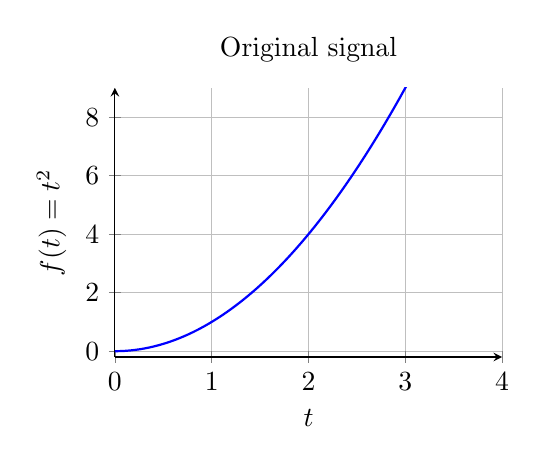
\begin{tikzpicture}
  % Left panel: f(t) = t^2
  \begin{axis}[
    width=6.5cm, height=5cm,
    xmin=0, xmax=4, ymin=-0.2, ymax=9,
    xlabel={$t$}, ylabel={$f(t)=t^2$},
    title={Original signal},
    grid=major,
    xtick={0,1,2,3,4},
    axis lines=left
  ]
    \addplot[blue, thick, domain=0:4, samples=80] {x^2};
  \end{axis}
\end{tikzpicture}
\hspace{1cm}
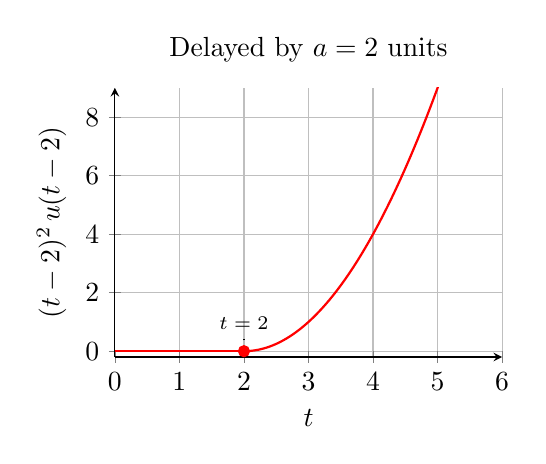
\begin{tikzpicture}
  % Right panel: (t-2)^2 * u(t-2)
  \begin{axis}[
    width=6.5cm, height=5cm,
    xmin=0, xmax=6, ymin=-0.2, ymax=9,
    xlabel={$t$}, ylabel={$(t-2)^2\,u(t-2)$},
    title={Delayed by $a=2$ units},
    grid=major,
    xtick={0,1,2,3,4,5,6},
    axis lines=left
  ]
    % Zero for t < 2
    \addplot[red, thick, domain=0:2, samples=2] {0};
    % Parabola for t >= 2
    \addplot[red, thick, domain=2:6, samples=80] {(x-2)^2};
    % Mark the jump point
    \addplot[red, only marks, mark=*, mark options={fill=red}] coordinates {(2,0)};
    \draw[dashed] (axis cs:2,-0.2) -- (axis cs:2,0.4) node[above, font=\scriptsize] {$t=2$};
  \end{axis}
\end{tikzpicture}
\end{center}

\begin{infobox}{Worked Example: Second Shifting Theorem}
\textbf{Find} $\mathcal{L}\{(t-2)^2\,u(t-2)\}$.

\emph{Step 1.} Identify: $f(t) = t^2$ and $a = 2$, so $f(t-2) = (t-2)^2$.

\emph{Step 2.} Look up the standard table: $\mathcal{L}\{t^2\} = \dfrac{2!}{s^3} = \dfrac{2}{s^3} = F(s)$.

\emph{Step 3.} Apply the Second Shifting Theorem:
\[
  \mathcal{L}\{(t-2)^2\,u(t-2)\} = e^{-2s}\,F(s) = \frac{2\,e^{-2s}}{s^3}.
\]

\textbf{Answer:} $\dfrac{2\,e^{-2s}}{s^3}$.
\end{infobox}

\begin{learnbox}{What Did We Learn?}
Delaying a signal by $a$ in the time domain multiplies its Laplace transform by $e^{-as}$.
Always include the $u(t-a)$ factor --- without it, the signal would not be zero before $t=a$,
and the Second Shifting Theorem would not apply.
\end{learnbox}

% ============================================================
\section{Property~3 --- Change of Scale}
% ============================================================

\begin{infobox}{Theorem: Change of Scale Property}
\textbf{Statement.} If $\mathcal{L}\{f(t)\} = F(s)$, then for any constant $a > 0$,
\[
  \mathcal{L}\{f(at)\} = \frac{1}{a}\,F\!\left(\frac{s}{a}\right).
\]

\textbf{Proof.}
\begin{align*}
  \mathcal{L}\{f(at)\}
  &= \int_0^{\infty} e^{-st}\,f(at)\,dt.
\end{align*}
Substitute $u = at$, so $t = u/a$ and $dt = du/a$:
\begin{align*}
  &= \int_0^{\infty} e^{-s(u/a)}\,f(u)\,\frac{du}{a}
   = \frac{1}{a}\int_0^{\infty} e^{-(s/a)\,u}\,f(u)\,du
   = \frac{1}{a}\,F\!\left(\frac{s}{a}\right). \qquad \checkmark
\end{align*}

\textbf{Worked example: } Given $\mathcal{L}\{\sin t\} = \dfrac{1}{s^2+1}$, find
$\mathcal{L}\{\sin(3t)\}$ using the Change of Scale property.

\emph{Step 1.} Here $f(t) = \sin t$ with $F(s) = \dfrac{1}{s^2+1}$, and $a = 3$.

\emph{Step 2.} Apply the property:
\[
  \mathcal{L}\{\sin(3t)\}
  = \frac{1}{3}\,F\!\left(\frac{s}{3}\right)
  = \frac{1}{3}\cdot\frac{1}{\left(\dfrac{s}{3}\right)^2 + 1}.
\]

\emph{Step 3.} Simplify the denominator:
\[
  \left(\frac{s}{3}\right)^2 + 1 = \frac{s^2}{9} + 1 = \frac{s^2 + 9}{9}.
\]

\emph{Step 4.} Substitute back:
\[
  \mathcal{L}\{\sin(3t)\}
  = \frac{1}{3}\cdot\frac{9}{s^2+9}
  = \frac{3}{s^2+9}. \quad \checkmark
\]
This agrees exactly with the standard table result $\mathcal{L}\{\sin(bt)\} = b/(s^2+b^2)$ at $b=3$.
\end{infobox}

\begin{learnbox}{What Did We Learn?}
Scaling time by $a$ (compressing or stretching the signal) scales the $s$-variable by $1/a$
and introduces an overall factor of $1/a$ in the transform. A larger $a$ (faster signal)
moves the transform energy to larger $s$-values.
\end{learnbox}

% ============================================================
\section{Property~4 --- Multiplication by $t^n$ (Introduction)}
% ============================================================

\begin{infobox}{Property: Multiplication by $t^n$}
\textbf{Statement.} If $\mathcal{L}\{f(t)\} = F(s)$, then
\[
  \mathcal{L}\{t^n f(t)\} = (-1)^n \frac{d^n}{ds^n}\,F(s), \quad n = 1, 2, 3, \ldots
\]
For $n=1$: $\displaystyle\mathcal{L}\{t\,f(t)\} = -\,F'(s) = -\frac{d}{ds}F(s)$.

(The full derivation appears in Topic~10. Here we use the result as a tool.)

\bigskip
\textbf{Worked example: } Find $\mathcal{L}\{t\sin(at)\}$.

\emph{Step 1.} Let $f(t) = \sin(at)$, so $F(s) = \dfrac{a}{s^2+a^2}$.

\emph{Step 2.} Apply the $n=1$ formula:
\[
  \mathcal{L}\{t\sin(at)\} = -\frac{d}{ds}\left[\frac{a}{s^2+a^2}\right].
\]

\emph{Step 3.} Differentiate using the quotient rule. Let $u = a$ (constant) and
$v = s^2+a^2$. Then $u'=0$, $v'=2s$:
\[
  \frac{d}{ds}\left[\frac{a}{s^2+a^2}\right]
  = \frac{0\cdot(s^2+a^2) - a\cdot 2s}{(s^2+a^2)^2}
  = \frac{-2as}{(s^2+a^2)^2}.
\]

\emph{Step 4.} Multiply by $-1$:
\[
  \mathcal{L}\{t\sin(at)\} = -\left(\frac{-2as}{(s^2+a^2)^2}\right) = \frac{2as}{(s^2+a^2)^2}.
\]
\end{infobox}

\begin{learnbox}{What Did We Learn?}
Multiplying $f(t)$ by $t$ corresponds to differentiating $F(s)$ and changing the sign. This
avoids computing $\int_0^\infty t\,f(t)\,e^{-st}\,dt$ from scratch. For $t^2$, differentiate
twice; for $t^3$, differentiate three times.
\end{learnbox}

% ============================================================
\section{Property~5 --- Division by $t$ (Introduction)}
% ============================================================

\begin{infobox}{Property: Division by $t$}
\textbf{Statement.} If $\mathcal{L}\{f(t)\} = F(s)$ and
$\displaystyle\lim_{t\to 0^+}\frac{f(t)}{t}$ exists (is finite), then
\[
  \mathcal{L}\!\left\{\frac{f(t)}{t}\right\} = \int_s^{\infty} F(u)\,du.
\]

(The full derivation is in Topic~11.)

\bigskip
\textbf{Worked example: } Given $\mathcal{L}\{\sin t\} = \dfrac{1}{s^2+1}$, find
$\mathcal{L}\!\left\{\dfrac{\sin t}{t}\right\}$.

\emph{Step 1.} Check the condition: $\displaystyle\lim_{t\to 0^+}\frac{\sin t}{t} = 1$.
The limit is finite, so the property applies.

\emph{Step 2.} Identify $F(u) = \dfrac{1}{u^2+1}$. Apply the division formula:
\[
  \mathcal{L}\!\left\{\frac{\sin t}{t}\right\}
  = \int_s^{\infty} \frac{du}{u^2+1}.
\]

\emph{Step 3.} Evaluate the integral. Recall
$\displaystyle\int \frac{du}{u^2+1} = \arctan(u) + C$:
\[
  \int_s^{\infty} \frac{du}{u^2+1}
  = \Big[\arctan(u)\Big]_s^{\infty}
  = \frac{\pi}{2} - \arctan(s).
\]

\textbf{Answer:} $\displaystyle\mathcal{L}\!\left\{\frac{\sin t}{t}\right\} = \frac{\pi}{2} - \arctan(s)$.
\end{infobox}

\begin{learnbox}{What Did We Learn?}
Dividing $f(t)$ by $t$ corresponds to integrating $F(s)$ from $s$ to $\infty$. Always verify
the existence condition first --- if $f(0^+) \neq 0$, the limit $f(t)/t$ diverges and the
property cannot be used directly.
\end{learnbox}

% ============================================================
\section{Summary Properties Table}
% ============================================================

The following table collects all five properties introduced in this topic, plus two additional
standard properties for completeness.

\vspace{0.5em}
\begin{center}
\begin{tabular}{@{}p{4.5cm}p{6cm}p{4.5cm}@{}}
\toprule
\textbf{Property Name} & \textbf{Formula} & \textbf{Notes / Validity} \\
\midrule
Linearity &
  $\mathcal{L}\{\alpha f(t)+\beta g(t)\} = \alpha F(s)+\beta G(s)$ &
  Always valid \\
\midrule
First Shifting (s-shift) &
  $\mathcal{L}\{e^{at}f(t)\} = F(s-a)$ &
  $s > s_0 + a$ \\
\midrule
Second Shifting (t-shift) &
  $\mathcal{L}\{f(t-a)\,u(t-a)\} = e^{-as}F(s)$ &
  $a \geq 0$ \\
\midrule
Change of Scale &
  $\mathcal{L}\{f(at)\} = \dfrac{1}{a}F\!\left(\dfrac{s}{a}\right)$ &
  $a > 0$ \\
\midrule
Multiplication by $t^n$ &
  $\mathcal{L}\{t^n f(t)\} = (-1)^n F^{(n)}(s)$ &
  $n = 1, 2, 3, \ldots$ \\
\midrule
Division by $t$ &
  $\mathcal{L}\!\left\{\dfrac{f(t)}{t}\right\} = \displaystyle\int_s^{\infty} F(u)\,du$ &
  $\lim_{t\to 0^+}\dfrac{f(t)}{t}$ must exist \\
\midrule
Transform of Derivative &
  $\mathcal{L}\{f'(t)\} = sF(s) - f(0)$ &
  Requires $f$ piecewise smooth \\
\midrule
Transform of Integral &
  $\mathcal{L}\!\left\{\int_0^t f(\tau)\,d\tau\right\} = \dfrac{F(s)}{s}$ &
  Valid for $s > 0$ \\
\bottomrule
\end{tabular}
\end{center}
\vspace{0.5em}

% ============================================================
\section{Worked Examples}
% ============================================================

\subsection*{Example 1 --- First Shifting Theorem}

\begin{infobox}{Example 1: Find $\mathcal{L}\{e^{-2t}\cos(3t)\}$}
\textbf{Strategy:} Use the First Shifting Theorem with $a = -2$ and $f(t) = \cos(3t)$.

\emph{Step 1.} Look up the standard table:
\[
  \mathcal{L}\{\cos(3t)\} = \frac{s}{s^2+9} = F(s).
\]

\emph{Step 2.} Apply First Shifting Theorem --- replace every $s$ by $(s-(-2)) = (s+2)$:
\[
  \mathcal{L}\{e^{-2t}\cos(3t)\} = F(s+2) = \frac{s+2}{(s+2)^2+9}.
\]

\emph{Step 3.} Expand the denominator for clarity:
\[
  (s+2)^2 + 9 = s^2 + 4s + 4 + 9 = s^2 + 4s + 13.
\]

\textbf{Final Answer:}
\[
  \mathcal{L}\{e^{-2t}\cos(3t)\} = \frac{s+2}{s^2+4s+13}.
\]
\end{infobox}

\begin{learnbox}{What Did We Learn?}
When $a$ is \emph{negative} (decay, e.g., $e^{-2t}$), the shift goes to the \emph{left} in the complex $s$-plane (replace $s$ by $s+|a|$).
The denominator becomes a completed square, which is the fingerprint of cosine (or sine) shifted.
\end{learnbox}

\subsection*{Example 2 --- Second Shifting Theorem with Piecewise Function}

\begin{infobox}{Example 2: Piecewise function via unit step, then Laplace transform}
Given:
\[
  f(t) = \begin{cases} 0 & 0 \leq t < 1, \\ t-1 & t \geq 1. \end{cases}
\]

\emph{Step 1. Express using unit step function.}
The function switches from 0 to $(t-1)$ at $t = 1$. We write:
\[
  f(t) = (t-1)\,u(t-1).
\]
Verification: for $t < 1$, $u(t-1) = 0$ so $f(t) = 0$. For $t \geq 1$, $u(t-1) = 1$ so
$f(t) = t-1$. \checkmark

\emph{Step 2. Identify the shifted function.}
Here $g(t) = t$, shifted by $a = 1$: $g(t-1) = t-1$.
From the table: $\mathcal{L}\{g(t)\} = \mathcal{L}\{t\} = \dfrac{1}{s^2} = G(s)$.

\emph{Step 3. Apply the Second Shifting Theorem.}
\[
  \mathcal{L}\{(t-1)\,u(t-1)\} = e^{-s}\,G(s) = \frac{e^{-s}}{s^2}.
\]

\textbf{Final Answer:} $\mathcal{L}\{f(t)\} = \dfrac{e^{-s}}{s^2}$.
\end{infobox}

\begin{learnbox}{What Did We Learn?}
Any piecewise function that ``turns on'' at $t = a$ can be written as $g(t-a)\,u(t-a)$ for
an appropriate $g$. Once in that form, the Second Shifting Theorem gives the Laplace transform
in one step.
\end{learnbox}

\subsection*{Example 3 --- First Shifting Theorem applied to $t^2$}

\begin{infobox}{Example 3: Find $\mathcal{L}\{t^2 e^{-t}\}$}
\textbf{Strategy:} Use the First Shifting Theorem with $a = -1$ and $f(t) = t^2$.

\emph{Step 1.} Standard table entry:
\[
  \mathcal{L}\{t^2\} = \frac{2!}{s^3} = \frac{2}{s^3} = F(s).
\]

\emph{Step 2.} Apply First Shifting Theorem with $a = -1$
(i.e., replace $s$ by $s-(-1) = s+1$):
\[
  \mathcal{L}\{t^2 e^{-t}\} = F(s+1) = \frac{2}{(s+1)^3}.
\]

\emph{Step 3.} No further simplification is needed; the answer is already compact.

\textbf{Final Answer:}
\[
  \mathcal{L}\{t^2 e^{-t}\} = \frac{2}{(s+1)^3}.
\]
\end{infobox}

\begin{learnbox}{What Did We Learn?}
For $e^{at}t^n$, the Laplace transform is always $n!/(s-a)^{n+1}$. The First Shifting Theorem
makes this a one-step substitution from the $t^n$ table entry, regardless of $n$.
\end{learnbox}

% ============================================================
\section{Excel Example }
% ============================================================

\textbf{Objective:} Numerically verify the First Shifting Theorem for
$\mathcal{L}\{e^{2t}\sin(t)\}$ at $s = 4$.

The theorem predicts:
\[
  \mathcal{L}\{e^{2t}\sin(t)\}\Big|_{s=4}
  = \frac{1}{(4-2)^2 + 1} = \frac{1}{4+1} = \frac{1}{5} = 0.2.
\]

We approximate the Laplace integral
$\displaystyle\int_0^{\infty} e^{-4t}\,e^{2t}\sin(t)\,dt
= \int_0^{\infty} e^{-2t}\sin(t)\,dt$
numerically using a Riemann sum with step $\Delta t = 0.1$.

\vspace{0.5em}
\begin{center}
\small
\begin{tabular}{@{}ccccc@{}}
\toprule
\textbf{Col A} & \textbf{Col B} & \textbf{Col C} & \textbf{Col D} & \textbf{Col E} \\
$t$ & Integrand $e^{-4t}e^{2t}\sin t$ & Approx.~(B$\times$0.1) & Running Sum & Exact (0.2) \\
\midrule
0.0 & \texttt{=EXP(-4*A2)*EXP(2*A2)*SIN(A2)} & \texttt{=B2*0.1} & \texttt{=C2} & 0.2 \\
0.1 & \texttt{=EXP(-4*A3)*EXP(2*A3)*SIN(A3)} & \texttt{=B3*0.1} & \texttt{=D2+C3} & 0.2 \\
0.2 & \texttt{=EXP(-4*A4)*EXP(2*A4)*SIN(A4)} & \texttt{=B4*0.1} & \texttt{=D3+C4} & 0.2 \\
0.3 & \texttt{=EXP(-4*A5)*EXP(2*A5)*SIN(A5)} & \texttt{=B5*0.1} & \texttt{=D4+C5} & 0.2 \\
0.4 & \texttt{=EXP(-4*A6)*EXP(2*A6)*SIN(A6)} & \texttt{=B6*0.1} & \texttt{=D5+C6} & 0.2 \\
$\vdots$ & $\vdots$ & $\vdots$ & $\vdots$ & 0.2 \\
6.0 & \texttt{=EXP(-4*A62)*EXP(2*A62)*SIN(A62)} & \texttt{=B62*0.1} & \texttt{=D61+C62} & 0.2 \\
\bottomrule
\end{tabular}
\end{center}
\vspace{0.5em}

\textbf{How to set up the spreadsheet:}
\begin{enumerate}
  \item In column~A, enter $t = 0.0$ in cell A2, then $t = 0.1$ in A3. Select A2:A3 and
        drag down to row~62 (covering $t = 0.0$ to $t = 6.0$).
  \item In column~B (cell B2), enter: \texttt{=EXP(-4*A2)*EXP(2*A2)*SIN(A2)} and drag down.
        This computes the integrand $e^{-4t}\cdot e^{2t}\cdot\sin(t) = e^{-2t}\sin(t)$.
  \item In column~C (cell C2), enter \texttt{=B2*0.1} (rectangle width $\Delta t = 0.1$)
        and drag down. This is each rectangle's area.
  \item In column~D (cell D2), enter \texttt{=C2}; in D3 enter \texttt{=D2+C3}. Drag D3 down
        to row~62. Cell D62 is the running Riemann sum --- the numerical approximation.
  \item In column~E, place the exact value $0.2$ in every row for comparison.
\end{enumerate}

\textbf{Expected result:} The running sum in column~D should converge to approximately $0.200$
as $t$ increases, confirming that $1/((4-2)^2+1) = 0.2$.

\begin{learnbox}{What Did We Learn?}
The numerical integration confirms the First Shifting Theorem: $e^{-4t}\cdot e^{2t}\sin(t)
= e^{-2t}\sin(t)$, and the integral equals $1/5 = 0.2$, matching $1/((s-a)^2+b^2)$ at
$s=4$, $a=2$, $b=1$. Numerical verification builds confidence in the algebraic theorem.
\end{learnbox}

% ============================================================
\section{Python Example }
% ============================================================

\begin{lstlisting}[language=Python, caption={Verifying Laplace Transform Properties using SymPy}]
import sympy as sp

t, s, a, b, u = sp.symbols('t s a b u', positive=True)

# -------------------------------------------------------
# 1. FIRST SHIFTING THEOREM
#    L{e^{at} f(t)} should equal F(s-a)
# -------------------------------------------------------

def verify_first_shift(f_expr, label):
    """Compute L{e^{at}*f(t)} directly and compare to F(s-a)."""
    # Direct Laplace of e^{at}*f(t)
    direct = sp.laplace_transform(sp.exp(a*t) * f_expr, t, s, noconds=True)
    # Laplace of f(t) then substitute s -> s-a
    F_s    = sp.laplace_transform(f_expr, t, s, noconds=True)
    shifted = F_s.subs(s, s - a)
    match  = sp.simplify(direct - shifted) == 0
    print(f"{label}: direct={direct}, F(s-a)={shifted}, match={match}")

verify_first_shift(sp.cos(b*t), "f(t)=cos(bt)")
# Output: f(t)=cos(bt): direct=(s-a)/((s-a)^2+b^2), F(s-a)=(s-a)/((s-a)^2+b^2), match=True

verify_first_shift(t**2, "f(t)=t^2")
# Output: f(t)=t^2: direct=2/(s-a)^3, F(s-a)=2/(s-a)^3, match=True

verify_first_shift(sp.sin(b*t), "f(t)=sin(bt)")
# Output: f(t)=sin(bt): direct=b/((s-a)^2+b^2), F(s-a)=b/((s-a)^2+b^2), match=True

print()

# -------------------------------------------------------
# 2. CHANGE OF SCALE PROPERTY
#    L{f(at)} should equal (1/a)*F(s/a)
# -------------------------------------------------------

f_expr_scale = sp.exp(-t)   # f(t) = e^{-t}, so f(at) = e^{-at}
F_s_scale    = sp.laplace_transform(f_expr_scale, t, s, noconds=True)
# F(s) = 1/(s+1), so F(s/a) = 1/(s/a + 1) = a/(s+a)

# Direct: L{e^{-at}} = 1/(s+a)
direct_scale = sp.laplace_transform(sp.exp(-a*t), t, s, noconds=True)
# Property: (1/a)*F(s/a)
property_scale = sp.Rational(1,1)/a * F_s_scale.subs(s, s/a)

print("Change of Scale for f(t)=e^{-t}:")
print(f"  Direct L{{e^{{-at}}}}  = {sp.simplify(direct_scale)}")
# Output: Direct L{e^{-at}}  = 1/(a+s)
print(f"  (1/a)*F(s/a)      = {sp.simplify(property_scale)}")
# Output: (1/a)*F(s/a)      = 1/(a+s)
print(f"  Match: {sp.simplify(direct_scale - property_scale) == 0}")
# Output: Match: True
\end{lstlisting}

\begin{learnbox}{What Did We Learn?}
SymPy's \texttt{laplace\_transform} function confirms all three tests of the First Shifting
Theorem (for $\cos(bt)$, $t^2$, $\sin(bt)$) and the Change of Scale property (for $e^{-t}$).
Symbolic verification is an excellent way to cross-check hand calculations before an exam.
\end{learnbox}

% ============================================================
\section{Viva-Style Oral Questions}
% ============================================================

\begin{enumerate}

\item \textbf{State the First Shifting Theorem.}\\
\textbf{Answer.} If $\mathcal{L}\{f(t)\} = F(s)$, then $\mathcal{L}\{e^{at}f(t)\} = F(s-a)$
for $s > s_0 + a$. Multiplying a time-domain signal by $e^{at}$ is equivalent to shifting the
transform variable from $s$ to $s - a$.

\item \textbf{Outline the proof of the First Shifting Theorem.}\\
\textbf{Answer.} Write the Laplace integral:
$\mathcal{L}\{e^{at}f(t)\} = \int_0^\infty e^{-st}e^{at}f(t)\,dt
= \int_0^\infty e^{-(s-a)t}f(t)\,dt = F(s-a).$
The key step is combining the two exponentials into one, revealing that $s$ is simply replaced
by $s-a$ in the original transform.

\item \textbf{State the Second Shifting Theorem.}\\
\textbf{Answer.} If $\mathcal{L}\{f(t)\} = F(s)$ and $a \geq 0$, then
$\mathcal{L}\{f(t-a)\,u(t-a)\} = e^{-as}F(s).$
Delaying a signal by $a$ in the time domain multiplies the Laplace transform by $e^{-as}$.

\item \textbf{What does the unit step function $u(t-a)$ do in the Second Shifting Theorem?}\\
\textbf{Answer.} It ``switches on'' the delayed signal $f(t-a)$ at $t = a$ and keeps it
at zero for all $t < a$. Without $u(t-a)$, the function $f(t-a)$ would exist for $t < a$
(possibly with negative $t$ arguments), which violates causality and makes the theorem
inapplicable.

\item \textbf{Why does the factor $e^{-as}$ appear in the Second Shifting Theorem?}\\
\textbf{Answer.} It comes from the substitution $\tau = t - a$ in the integral
$\int_a^\infty e^{-st}f(t-a)\,dt$. After substituting, $t = \tau + a$, so
$e^{-st} = e^{-s(\tau+a)} = e^{-sa}\,e^{-s\tau}$. The factor $e^{-sa}$ (constant w.r.t.
$\tau$) comes outside the integral, yielding $e^{-as}F(s)$.

\item \textbf{State the Change of Scale property and give the formula.}\\
\textbf{Answer.} If $\mathcal{L}\{f(t)\} = F(s)$ and $a > 0$, then
$\mathcal{L}\{f(at)\} = \tfrac{1}{a}F(s/a).$
Compressing time by a factor $a$ stretches the transform by $a$ (argument $s$ becomes $s/a$)
and reduces the overall amplitude by $1/a$.

\item \textbf{State the Multiplication by $t$ property.}\\
\textbf{Answer.} If $\mathcal{L}\{f(t)\} = F(s)$, then $\mathcal{L}\{t\,f(t)\} = -F'(s).$
More generally, $\mathcal{L}\{t^n f(t)\} = (-1)^n F^{(n)}(s).$ Each multiplication by $t$
corresponds to one differentiation of the transform and a sign change.

\item \textbf{When is the Division by $t$ property valid?}\\
\textbf{Answer.} The property $\mathcal{L}\{f(t)/t\} = \int_s^\infty F(u)\,du$ holds if and only
if $\displaystyle\lim_{t\to 0^+}\frac{f(t)}{t}$ is finite. For example, $f(t) = \sin t$ satisfies
this since $\sin(t)/t \to 1$ as $t \to 0^+$. But $f(t) = t^{-1/2}$ does not, because
$t^{-1/2}/t = t^{-3/2} \to \infty$.

\end{enumerate}

% ============================================================
\section{Descriptive Questions}
% ============================================================

\begin{enumerate}

\item \textbf{State and prove the First Shifting Theorem.}\\
State: If $\mathcal{L}\{f(t)\} = F(s)$, then $\mathcal{L}\{e^{at}f(t)\} = F(s-a)$.
Proof: $\int_0^\infty e^{-st}e^{at}f(t)\,dt = \int_0^\infty e^{-(s-a)t}f(t)\,dt = F(s-a).$
Explain the domain constraint $s > s_0 + a$ and give two applications from the standard table.

\item \textbf{State and prove the Second Shifting Theorem.}\\
State: If $\mathcal{L}\{f(t)\} = F(s)$ and $a \geq 0$, then
$\mathcal{L}\{f(t-a)\,u(t-a)\} = e^{-as}F(s)$.
Proof: Split the integral at $t = a$, substitute $\tau = t - a$, and factor out $e^{-as}$.
Explain the role of the unit step function.

\item \textbf{Derive the Change of Scale property.}\\
Starting from the definition $\mathcal{L}\{f(at)\} = \int_0^\infty e^{-st}f(at)\,dt$,
substitute $u = at$ to obtain $\tfrac{1}{a}F(s/a)$. Show every algebraic step and
verify the result using $f(t) = e^{-t}$ (so $f(at) = e^{-at}$ and $F(s) = 1/(s+1)$).

\item \textbf{Find $\mathcal{L}\{te^{at}\}$ using the Multiplication by $t$ property.}\\
Let $f(t) = e^{at}$ with $\mathcal{L}\{e^{at}\} = 1/(s-a) = F(s)$.
By the property: $\mathcal{L}\{t\cdot e^{at}\} = -F'(s) = -\frac{d}{ds}\left[\frac{1}{s-a}\right]
= \frac{1}{(s-a)^2}.$ Show the differentiation in full. Confirm for $a=0$:
$\mathcal{L}\{t\} = 1/s^2$. \checkmark

\item \textbf{Find $\mathcal{L}\{(1-\cos t)/t\}$ using the Division by $t$ property.}\\
Let $f(t) = 1 - \cos t$. Check: $\lim_{t\to 0^+}(1-\cos t)/t = 0$ (finite). So the property
applies.
$F(s) = \mathcal{L}\{1-\cos t\} = 1/s - s/(s^2+1).$
Then $\mathcal{L}\{(1-\cos t)/t\} = \int_s^\infty \left(\frac{1}{u} - \frac{u}{u^2+1}\right)du
= \Big[\ln u - \tfrac{1}{2}\ln(u^2+1)\Big]_s^\infty
= \tfrac{1}{2}\ln\!\left(1 + \tfrac{1}{s^2}\right).$

\end{enumerate}

% ============================================================
\section{Practice Problems}
% ============================================================

\begin{enumerate}

\item Find $\mathcal{L}\{e^{-3t}t^2\}$.\\
\textit{Hint:} Use First Shifting Theorem with $f(t)=t^2$, $a=-3$.
\textit{Answer:} $2/(s+3)^3$.

\item Find $\mathcal{L}\{e^{t}\cos(2t)\}$.\\
\textit{Hint:} $\mathcal{L}\{\cos(2t)\}=s/(s^2+4)$; shift $s\to s-1$.
\textit{Answer:} $(s-1)/\bigl((s-1)^2+4\bigr)$.

\item Find $\mathcal{L}\{(t-1)\,u(t-1)\}$.\\
\textit{Hint:} Second Shifting Theorem with $f(t)=t$, $a=1$.
\textit{Answer:} $e^{-s}/s^2$.

\item Find $\mathcal{L}\{t\cos(at)\}$ using the Multiplication by $t$ property.\\
\textit{Hint:} $F(s)=s/(s^2+a^2)$; compute $-F'(s)$.
\textit{Answer:} $(s^2-a^2)/(s^2+a^2)^2$.

\item Find $\mathcal{L}\{(e^{at}-1)/t\}$ using the Division by $t$ property.\\
\textit{Hint:} $\mathcal{L}\{e^{at}-1\}=1/(s-a)-1/s$; integrate from $s$ to $\infty$.
\textit{Answer:} $\ln\!
\bigl(s/(s-a)\bigr)$ (valid for $s > a > 0$).

\item Find $\mathcal{L}\{\sin(2t + \pi/3)\}$.\\
\textit{Hint:} Expand using the angle-addition formula:
$\sin(2t+\pi/3) = \sin(2t)\cos(\pi/3)+\cos(2t)\sin(\pi/3)
= \tfrac{1}{2}\sin(2t) + \tfrac{\sqrt{3}}{2}\cos(2t)$;
then apply linearity and the standard table.
\textit{Answer:} $\dfrac{1}{2}\cdot\dfrac{2}{s^2+4}+\dfrac{\sqrt{3}}{2}\cdot\dfrac{s}{s^2+4}
= \dfrac{2+\sqrt{3}s}{2(s^2+4)}$.

\end{enumerate}

% ============================================================
\section{MCQs}
% ============================================================

\begin{enumerate}

\item If $\mathcal{L}\{\sin(bt)\} = b/(s^2+b^2)$, then $\mathcal{L}\{e^{at}\sin(bt)\}$ equals:\\
(a) $\dfrac{b}{(s+a)^2+b^2}$ \quad
\textbf{(b) $\dfrac{b}{(s-a)^2+b^2}$} \quad
(c) $\dfrac{b}{s^2+b^2}\,e^{-as}$ \quad
(d) $\dfrac{b}{(s^2-a^2)+b^2}$\\
\textit{Explanation:} First Shifting Theorem replaces $s$ by $s - a$, giving option (b).

\item The Laplace transform $\mathcal{L}\{f(t-a)\,u(t-a)\}$ equals:\\
(a) $F(s)$ \quad
(b) $e^{as}F(s)$ \quad
\textbf{(c) $e^{-as}F(s)$} \quad
(d) $F(s-a)$\\
\textit{Explanation:} Second Shifting Theorem: delaying by $a$ introduces $e^{-as}$ (negative sign).

\item If $\mathcal{L}\{f(t)\} = F(s)$ and $a > 0$, then $\mathcal{L}\{f(at)\}$ equals:\\
(a) $a\,F(as)$ \quad
\textbf{(b) $\dfrac{1}{a}\,F\!\left(\dfrac{s}{a}\right)$} \quad
(c) $F(as)$ \quad
(d) $\dfrac{1}{a}\,F(as)$\\
\textit{Explanation:} Change of Scale: both the $1/a$ factor and the $s/a$ argument are required.

\item Using Multiplication by $t$, $\mathcal{L}\{t\,e^{at}\}$ equals:\\
(a) $\dfrac{1}{(s-a)}$ \quad
(b) $\dfrac{1}{(s-a)^3}$ \quad
\textbf{(c) $\dfrac{1}{(s-a)^2}$} \quad
(d) $\dfrac{2}{(s-a)^3}$\\
\textit{Explanation:} $-\dfrac{d}{ds}\left[\dfrac{1}{s-a}\right] = \dfrac{1}{(s-a)^2}$.

\item In the Second Shifting Theorem $\mathcal{L}\{f(t-a)\,u(t-a)\} = e^{-as}F(s)$,
the factor $e^{-as}$ arises because:\\
(a) $e^{-as}$ is the Laplace transform of $e^{-at}$ \quad
(b) the theorem uses complex frequency $s+a$ \quad
\textbf{(c) substituting $\tau = t-a$ introduces $e^{-as}$ as a constant factor outside the integral} \quad
(d) the unit step function contributes $e^{-as}$ independently\\
\textit{Explanation:} After substitution $\tau = t-a$, the term $e^{-s(\tau+a)} = e^{-as}e^{-s\tau}$;
the $e^{-as}$ factor is constant and comes out of the integral, giving $e^{-as}F(s)$.

\end{enumerate}

% ============================================================
\section{Common Mistakes}
% ============================================================

\begin{mistakebox}{Common Mistakes in Properties of Laplace Transforms}
\begin{tabular}{@{}p{4cm}p{4.5cm}p{5cm}@{}}
\toprule
\textbf{Mistake} & \textbf{What Students Do} & \textbf{Correct Approach} \\
\midrule
Shifting $t$ instead of $s$ &
  Write $\mathcal{L}\{e^{at}f(t)\} = e^{-as}F(s)$ (confusing with Second Shifting) &
  First Shifting: replace $s$ by $s-a$ in $F(s)$; never multiply by $e^{-as}$ \\
\midrule
Forgetting $u(t-a)$ in the inverse &
  Write $\mathcal{L}^{-1}\{e^{-as}F(s)\} = f(t-a)$ (missing the unit step) &
  Always write $f(t-a)\,u(t-a)$; the step function is part of the answer \\
\midrule
Change of Scale without $1/a$ factor &
  Write $\mathcal{L}\{f(at)\} = F(s/a)$ (omitting the $1/a$ prefactor) &
  The correct formula is $\mathcal{L}\{f(at)\} = \tfrac{1}{a}F(s/a)$ \\
\midrule
Using Division by $t$ without checking limit &
  Apply $\mathcal{L}\{f(t)/t\} = \int_s^\infty F(u)\,du$ when $f(0^+)/0$ is undefined &
  First verify $\lim_{t\to 0^+} f(t)/t$ exists; if not, the property cannot be applied \\
\midrule
Sign error in First Shifting &
  Use $F(s+a)$ instead of $F(s-a)$ when $a > 0$ &
  Multiplying by $e^{at}$ shifts \emph{left} by $a$ in $s$ (replace $s$ by $s-a$, not $s+a$) \\
\bottomrule
\end{tabular}
\end{mistakebox}

% ============================================================
\section{Quick Recap}
% ============================================================

\begin{learnbox}{Quick Recap --- Properties of Laplace Transforms}
\begin{itemize}
  \item \textbf{First Shifting (s-shift):}
        $\mathcal{L}\{e^{at}f(t)\} = F(s-a)$ --- replace $s$ with $s-a$.
  \item \textbf{Second Shifting (t-shift):}
        $\mathcal{L}\{f(t-a)\,u(t-a)\} = e^{-as}F(s)$ --- always include $u(t-a)$.
  \item \textbf{Change of Scale:}
        $\mathcal{L}\{f(at)\} = \tfrac{1}{a}F(s/a)$ --- both the factor $1/a$ and the argument
        $s/a$ are required.
  \item \textbf{Multiplication by $t^n$:}
        $\mathcal{L}\{t^n f(t)\} = (-1)^n F^{(n)}(s)$ --- differentiate $F(s)$ $n$ times and
        multiply by $(-1)^n$.
  \item \textbf{Division by $t$:}
        $\mathcal{L}\{f(t)/t\} = \int_s^\infty F(u)\,du$ --- only valid when
        $\lim_{t\to 0^+}f(t)/t$ is finite.
  \item \textbf{s-shift vs.~t-shift:} $s$-shifting multiplies by $e^{at}$ in time;
        $t$-shifting multiplies by $e^{-as}$ in frequency.
  \item \textbf{Unit step function key:} $u(t-a)$ is \emph{always} part of the answer for
        Second Shifting --- forgetting it is the most common exam error.
  \item \textbf{Use the summary table:} Keep the 8-row properties table handy during problem
        solving --- it covers all scenarios in this topic.
\end{itemize}
\end{learnbox}

\end{document}
